\chapter{原子核的组成}

\section{历程} 

\begin{enumerate}
    \item 电子的发现 
    \item 原子核的发现 $\rightarrow$卢瑟福用$\alpha$轰击金箔,有八千分之一的几率被反射。 $\Rightarrow$ 正电荷和原子质量几种在原子中心。
    \item 质子的发现 $\rightarrow$用$\alpha$粒子轰击$^{14}N$,发现了质子。($\alpha +  ^{14}_{7}N \Rightarrow  ^{17}_{8}O + p$)
    \item 早期原子核组成的想法及其碰到的困难
    \item 中子的发现 $\alpha + ^{9}Be \Rightarrow ^{12}C + n$  ,用n再打石蜡能出来质子,根据打出质子的能量,推测出不是射线,是中子(质量跟质子差不多)(不带电粒子的发现比较困难,因为电磁学知识已经完备,探测带电粒子比较简单)【中子穿透性强,寿命短~14.81min,可以用来做中子弹】
\end{enumerate}

\vspace{1.2em}

\textbf{原子核的符号表示:}$_{z}^{A}X_{n}$,z是质子数,A是核子数,N为中子数

\section{质子和中子的性质对比} 

\begin{enumerate}
    \item 中子比质子质量大一点点  938$MeV/c^2$  939$MeV/c^2$
    \item 统计性规律都是费米子
    \item 质子寿命非常长,$10^{31}$year,中子很短,14.81min。
    \item 随之探测技术发展,中子带一点点负电$(-0.4\pm 1.1)*10^{-23}e$(质子带$1\pm10^{-21}e$,中子带电比质子小两个数量级),可以认为不带电。
\end{enumerate}

\begin{figure}[htbp]
    \centering
    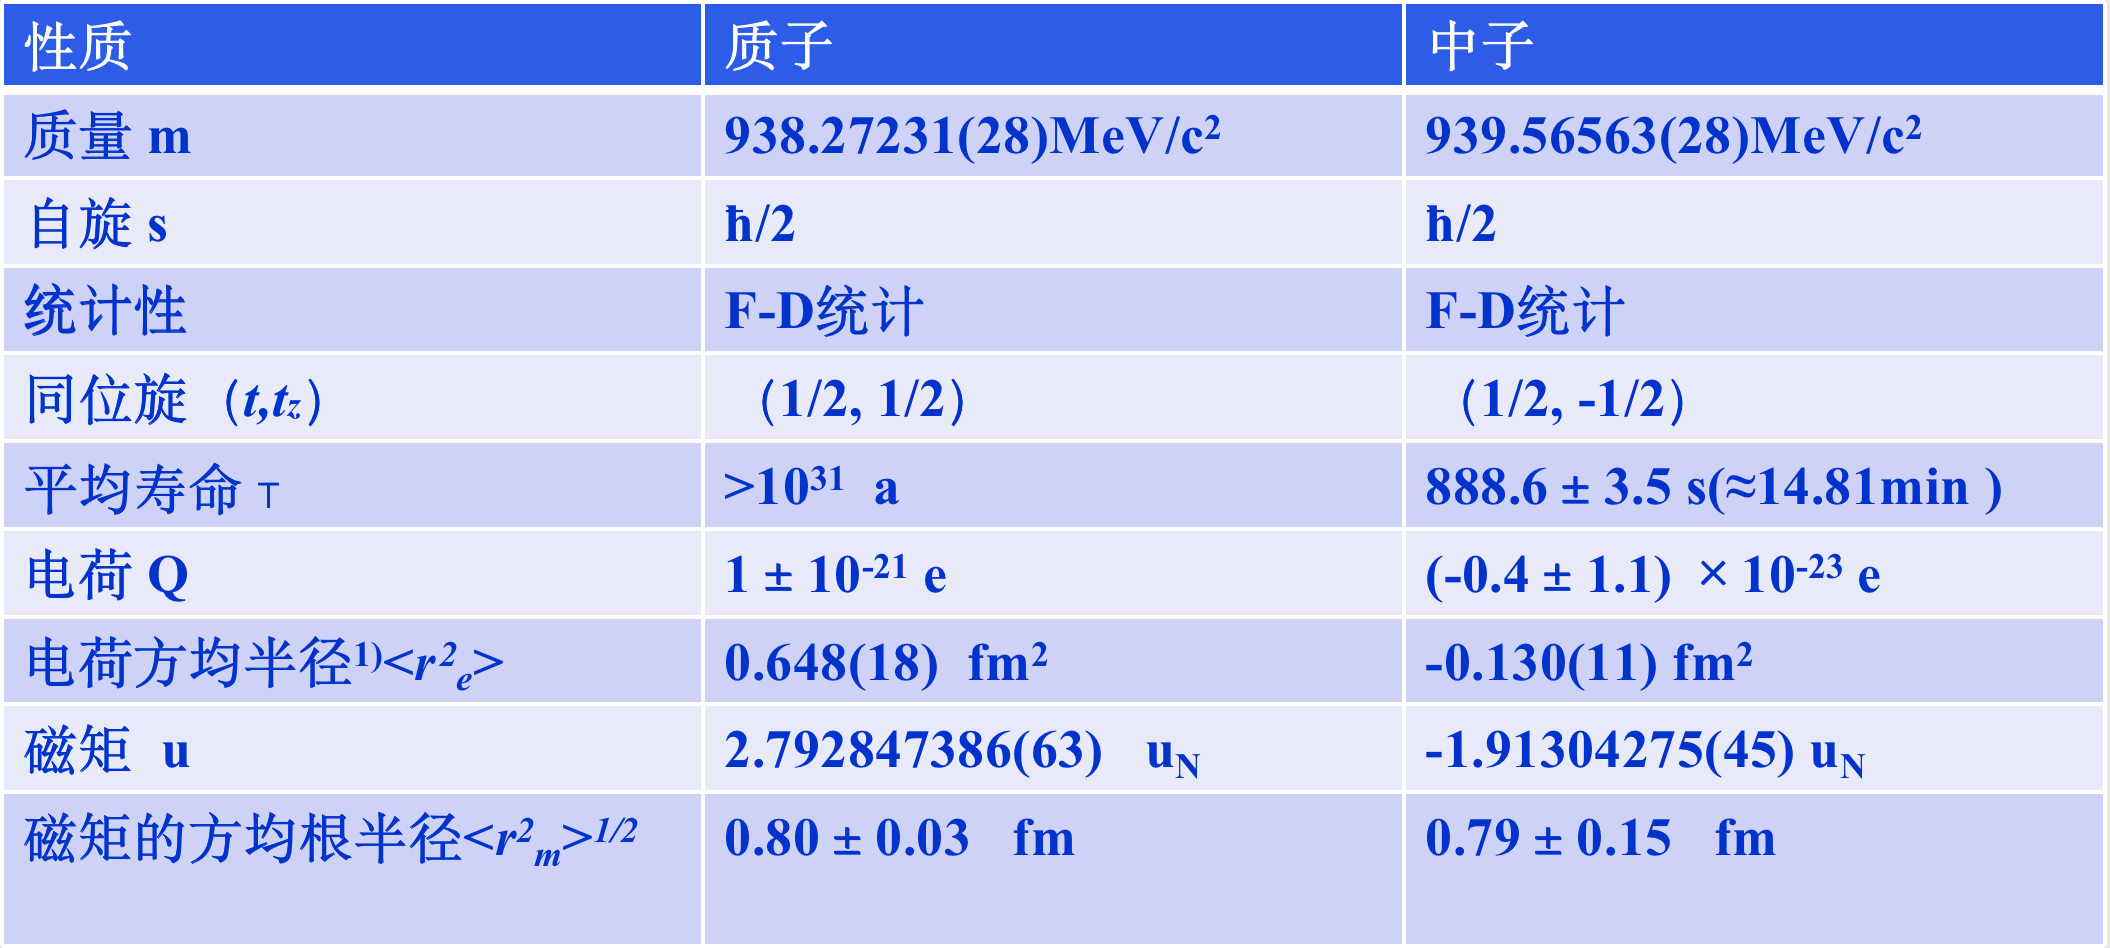
\includegraphics[width=14cm]{figure//fig001.png}
    \caption{\label{fig001}质子与中子的对比。}
\end{figure}

\section{亚核子自由度}

\textbf{实验猜想原子核内部质子中子是怎么分布的:}参考卢瑟福$\alpha$散射实验,使用小的$\alpha$粒子打大的金箔,根据$\alpha$粒子的散射情况,猜测原子的结构;这里使用电子打原子核,根据电子的散射情况,猜测原子核的结构。(这种实验方法叫电子散射)

如图~\ref{fig002}~所示,横坐标可以理解为距离质子/中子中心的距离,纵坐标表示电荷量。通过这个图,可以猜测出质子/中子并不是最小微粒,因为电荷分布不均匀。

\begin{figure}[htbp]
    \centering
    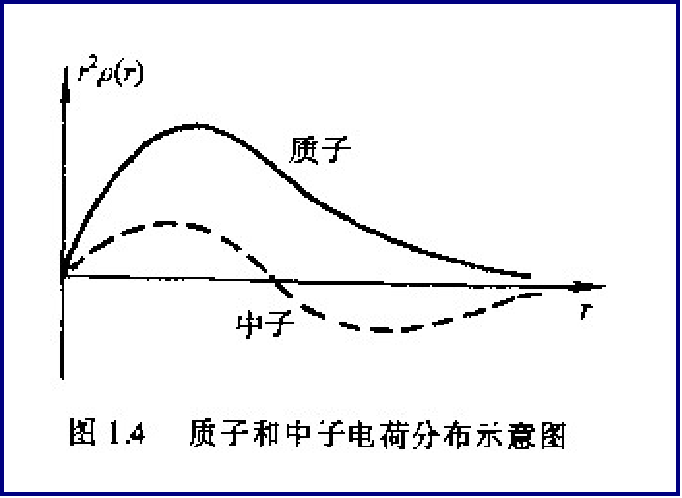
\includegraphics[width=14cm]{figure//fig002.png}
    \caption{\label{fig002}质子和中子电荷分布示意图。}
\end{figure}

\textbf{电子散射:}用电子轰击原子核,来推测原子核内部结构。

\textbf{质子和中子电荷分布示意图:}表明质子和中子并不是最微观的粒子。

\section{夸克}

质子和中子由夸克组成,总共有6种夸克:上夸克(up)、下夸克(down)、顶夸克(top)、底夸克(bottom)、粲夸克(charm)、奇异夸克(strange)。其中up/top/charm带三分之二的正电荷,dowm/bottom/strange带三分之一的负电荷。

质子和中子是费米子,夸克也是费米子。

质子由三个夸克组成,uud(两个up,一个down)

中子由三个夸克组成,ddu(两个down,一个up)

\section{夸克禁闭}

带色的粒子不能单独存在,夸克总是和别的夸克禁闭在一起而形成色中性的强子。

强子中的夸克疯狂的交换胶子进行强作用,他们存在于由胶子组成的色场中:当胶子场获得足够能量时,就会折断成一对夸克-反夸克。

夸克禁闭问题至今还没有完全解决清楚。

遗留问题:核子质量大约是电子1800倍,而核子由三个夸克组成,则电子不是由夸克组成,猜想还有比夸克更小的粒子。

\section{轻子}

总共6种轻子:e(电子)、$\tau$($\tau$子)、$\mu$ ($\mu$子)、Ve(电子中微子)、V$\tau$($\tau$子中微子)、V$\tau$($\mu$子中微子)

粒子物理标准模型:6种夸克+6种轻子+传递力的粒子

\clearpage
